\documentclass{llncs}
\usepackage{amsmath, amssymb, fancyvrb, multirow, color}
\usepackage{svg}
\usepackage{graphicx}
\usepackage{fancyvrb}

\newcommand{\dReal}{\textsf{dReal}}
\newcommand{\dReach}{\textsf{dReach}}

%\usepackage{multirow}
\usepackage{amsmath,hyperref}
\hypersetup{
    colorlinks,%
    citecolor=blue,%
    filecolor=blue,%
    linkcolor=blue,%
    urlcolor=blue
}
\usepackage{amssymb,verbatim}
\usepackage{fix2col,listings,fancyvrb}
\usepackage{multicol}
\usepackage{graphicx,epsfig}
\usepackage{caption}
\usepackage{stmaryrd}
\usepackage{setspace}
\usepackage{ulem}
\usepackage{newlfont}
\usepackage{epsfig,graphics}
\usepackage{fancybox}
\usepackage{listings}
\usepackage{caption}
\usepackage{graphicx,epsfig}
\usepackage{caption}
\usepackage{makeidx}
\usepackage{algorithm}
\usepackage{algpseudocode}
\usepackage{listings}
\lstset{
  basicstyle=\ttfamily,
  breaklines=true,
  columns=fullflexible,
  escapeinside = ||,
  breakindent=0pt}
\makeindex

\usepackage{algorithm}
\usepackage{algpseudocode}
\usepackage{hyperref}
\hypersetup{
    colorlinks,%
    citecolor=blue,%
    filecolor=blue,%
    linkcolor=blue,%
    urlcolor=blue
}
\usepackage{multicol}
\usepackage{lipsum}

\newtheorem{theorem}{Theorem}
\newtheorem{proofoutline}[theorem]{Proof Outline}
\newtheorem{lemma}[theorem]{Lemma}
\newtheorem{claim}[theorem]{Claim}
\newtheorem{proposition}[theorem]{Proposition}
\newtheorem{corollary}[theorem]{Corollary}
\newtheorem{fact}[theorem]{Fact}
\newtheorem{definition}[theorem]{Definition}
\newtheorem{remark}[theorem]{Remark}
\newtheorem{conjecture}[theorem]{Conjecture}
\newtheorem{example}[theorem]{Example}
\newtheorem{notation}[theorem]{Notation}
\newtheorem{question}[theorem]{Question}



%\usepackage[ruled,lined,boxed,commentsnumbered,linesnumbered]{algorithm2e}

\setcounter{secnumdepth}{3}
\setcounter{tocdepth}{2}

\newcommand\bookepigraph[4]{
\vspace{1em}\hfill{}\begin{minipage}{#1}{\begin{spacing}{0.9}
\small\noindent\textit{#2}\end{spacing}
\vspace{1em}
\hfill{}{#3}\\

\vspace{-1em}\begin{flushright}{#4}\end{flushright}}\vspace{2em}
\end{minipage}}

\newcommand{\dom}{\mbox{dom}}

\newcommand\epigraph[3]{
\vspace{1em}\hfill{}\begin{minipage}{#1}{\begin{spacing}{0.9}
\small\noindent\textit{#2}\end{spacing}
\vspace{1em}
\hfill{}{#3}}\vspace{2em}
\end{minipage}}

\newcommand\anonymousepigraph[2]{
\vspace{1em}\hfill{}\begin{minipage}{#1}{\begin{spacing}{0.9}
\small\noindent\textit{#2}\end{spacing}}
\vspace{1em}
\end{minipage}}

\newcommand{\len}{\mathit{len}}
\newcommand{\poly}{\mathsf{poly}}
\newcommand{\N}{\mathbb{N}}
\newcommand{\R}{\mathbb{R}}
\newcommand{\D}{\mathbb{D}}
\newcommand{\cf}{\mathsf{CF}}
\newcommand{\be}{\mathsf{BE}}
\newcommand{\fe}{\mathbb{F}^{[\underline{e}, \overline{e}]}_{\beta,p}}
\newcommand{\rad}{\mathrm{rad}}


\newcommand{\flow}{\mathsf{flow}}
\newcommand{\jump}{\mathsf{jump}}
\newcommand{\inv}{\mathsf{inv}}
\newcommand{\init}{\mathsf{init}}
\newcommand{\guard}{\mathsf{guard}}
\newcommand{\reset}{\mathsf{reset}}
\newcommand{\reach}{\mathsf{Reach}}
\newcommand{\unsafe}{\mathsf{unsafe}}

\newcommand{\safe}{\mathsf{safe}}
\newcommand{\p}{\mathsf{P}}
\newcommand{\np}{\mathsf{NP}}
%\newcommand{\dom}{\mathrm{dom}}


\newcommand\tupleof[1]{\left\langle #1 \right\rangle}
\newcommand\vI{\vec{I}}
\newcommand\va{\vec{a}}
\newcommand\vb{\vec{b}}
\newcommand\vc{\vec{c}}
\newcommand\vd{\vec{d}}
\newcommand\ve{\vec{e}}
\newcommand\vl{\vec{l}}
\newcommand\vu{\vec{u}}
\newcommand\vx{\vec{x}}
\newcommand\vy{\vec{y}}
\newcommand\trp[1]{#1^{{}^{\mbox{\sc{t}}}}}
\newcommand{\lrf}{\mathcal{L}_{\mathbb{R}_{\mathcal{F}}}}
%\usepackage{wrapfigure}

%\doublespacing


\title{\dReach{}: $\delta$-Complete Analysis Tool for Bounded Reachability of Hybrid Systems}

\begin{document}


\mainmatter  % start of an individual contribution

\author{Soonho Kong, Sicun Gao, Wei Chen, and Edmund Clarke}

\authorrunning{S. Kong, S. Gao, W. Chen,  E. Clarke}
\institute{Computer Science Department, Carnegie Mellon University, USA}
\maketitle

% Tool demonstration papers

% Submissions should consist of two parts:

% The first part, at most 4 pages, should describe the tool presented.
% Please include the URL of the tool (if available) and provide
% information that illustrates the maturity and robustness of the tool
% (this part will be included in the proceedings).

% The second part, at most 6 pages, should explain how the
% demonstration will be carried out and what it will show, including
% screen dumps and examples. (This part will be not be included in the
% proceedings, but will be evaluated.) ESOP and FOSSACS do not accept
% tool demonstration papers.

% TACAS has a page limit of 6 pages for tool demonstrations.

\section{Introduction}\label{sec:intro}

% Need a paragrapgh or two to explain why the tool is interesting and
% significant should be provided.

\dReach{} is a bounded model checker for hybrid systems. It encodes
bounded reachability problems of hybrid systems as first-order
formulas over the real numbers, and solves them using
$\delta$-decision procedures in the SMT solver \dReal{}. \dReach{} is
able to handle a wide range of highly nonlinear hybrid systems. It has
scaled well on various realistic nonlinear models from biomedical and
robotics applications~\cite{}.

It is well-known that the standard bounded reachability problems for
simple hybrid systems are already highly
undecidable~\cite{DBLP:conf/rex/AlurD91,DBLP:conf/hybrid/AlurCHH92}. In
previous work~\cite{}, we have defined the notion of
$\delta$-reachability problem of hybrid systems. In this new
framework, we have shown that bounded $\delta$-reachability is
decidable for a wide range of hybrid systems, with reasonable
complexity bounds~\cite{}. We give a brief review of the framework in
Section~\ref{sec:delta-reachability}.

Realistic hybrid systems involves nonlinear ODEs with transcendental
functions. \dReach{} allows users to specify a hybrid system in a
nonlinear signature as it is without linearizing or overapproximating
it. Users can provide the tool with a numerical error bound $\delta$,
a bounded time horizon $[0, T]$, and a maximum number of mode switches
$k$ for the analysis. As a result of analysis, \dReach{} will return
either \textbf{$\delta$-sat} with a concrete counterexample, or
\textbf{unsat} which does not involve numerical errors. We also
provide a visualization for the $\delta$-sat case to help
understand the analysis result.
\begin{figure}[!t]
  \subfloat[An example of nonlinear hybrid system model: off-treatment
  mode of the prostate cancer treatement model~\cite{}\label{subfig-1:prostate}]{
    \includegraphics[width=0.48\textwidth]{images/prostatebw-mode2.pdf}
  }
  \hfill
  \subfloat[Visualization of a concrete counterexample generated from
  dReach for the prostate cancer treatment model.]{%
    \includegraphics[width=0.48\textwidth]{images/prostate}
  }
  \caption{An example of nonlinear hybrid system model: Prostate
    cancer model.}
  \label{fig:prostate-example}
\end{figure}
For instance, figure~\ref{fig:prostate-example} shows a part of a
prostate cancer treatment model that contains nonlinear ODEs and a
visualization of a generated concrete counterexample.

\paragraph{Related Work}
%reachable set computation tools: flow star, SpaceX, Phaver,
%theorem provers:
%similar tools: iSAT, RSolver -- emphasize on the nonlinearity that we can handle.

The paper is structured as follows.


%%% Local Variables:
%%% mode: latex
%%% TeX-master: "main"
%%% End:

\section{System Description}

\begin{figure}
  \centering
  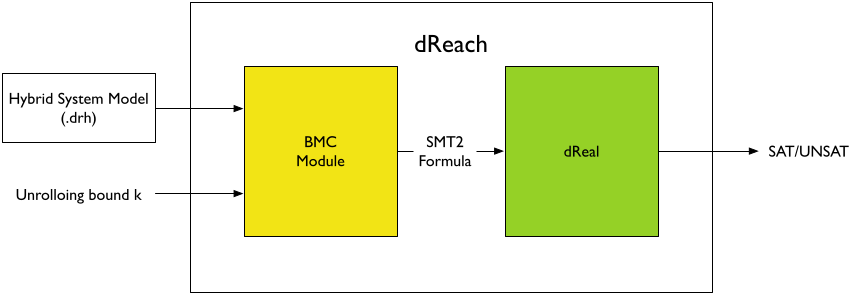
\includegraphics[width=\textwidth]{images/dReach}
  \caption{System Description of \dReach{}}
  \label{fig:system-description}
\end{figure}

Figure~\ref{fig:system-description} illustrates the architecture of
\dReach{}. We provide a domain-specific lanaguage to describe a hybrid
system and specify its safety properties. Given an input model,
specification, and unrolling bound $k$, \dReach{} reduces the
$\delta$-reachability problem to a $\delta$-decision problem of
formulas over the reals by providing a corresponding SMT encoding for
the problem. Then we answer the bounded reachability queries by using
our nonlinear SMT solver \dReal{}~\cite{DBLP:conf/cade/GaoKC13} to
solve the encoded problems.

\subsection{drh: a Language for Modeling and Specifying Hybrid Systems}

We define \texttt{drh}, a small language for describing hybrid systems
and specifying their initial and safety conditions. It consists of
five sections - macro definitions, variable declarations, mode
definitions, and initial condition, and goals.
\begin{align*}
  \textit{drh} := \ & \textit{macro-definition}^*\\
                  & \textit{variable-declaration}^+\\
                  & \textit{mode-definition}^+\\
                  & \textit{initial-condition}\\
                  & \textit{goal}^+
\end{align*}
In macro definitions, we allow users to define C-preprocessor macros
which can be used in following sections. Macros are expanded before
the other parts are processed.

A variable declaration has a form:
\[
\textit{variable-declaration} \ := \ \texttt{[}
                                     \textit{l}
                                     \texttt{,}
                                     \ \textit{u}
                                     \texttt{]}
                                     \ \textit{var}
                                     \texttt{;}
\]
and it declares a real variable $var$ whose domain is $[l, u] \in
\mathbb{IR}$. A special variable \textit{time} has to be delcared to
specify the time bound of bounded model checking.

A mode definition consists of mode id, mode invariant, flow, and jump.
\begin{align*}
  \textit{mode-definition} \ := & \ \texttt{\{}
                                    \texttt{mode} \ \textit{id}\texttt{;}\\
                           & \ \ \  \texttt{invt}:(\textit{formula} \texttt{;})^+\\
                           & \ \ \  \texttt{flow}:\textit{ode}^+\\
                           & \ \ \ \texttt{jump}:\textit{jump}^+ \texttt{\}}
\end{align*}
\textit{id} is a unique unsigned integer assigned to a mode. An
invariant is a conjuction of logic formulae which must hold in a mode.
A flow describes a continuous dynamics of a mode by providing a set of
ordinary differential equations (\textit{ode}s) which is a form of
``\texttt{d/dt[}\textit{x}\texttt{]=}\textit{exp}''. \textit{jump} is
a form of ``\textit{guard} \texttt{==>} \texttt{@}\textit{n}
\textit{reset}'' where \textit{guard} is a logic formula specifying a
condition to make a transition, $n$ is an id of target mode, and
\textit{reset} is a logic formula specifying the relationship between
old and new values.

\texttt{initial-condition} is of a form
``\texttt{@}\textit{mode-id} \textit{formula}\texttt{;}''
where \textit{mode-id} is an initial mode of a hybrid system and
\textit{formula} specifies the initial configuration of it.

\texttt{goal} shares the same syntactic structure,
``\texttt{@}\textit{mode-id} \textit{formula}\texttt{;}'' of
\textit{initial-condition} with a different interpretation. It poses a
reachability question: ``Is there a trajectory of a hybrid system
reaching \textit{mode-id} while satisfying the goal condition \textit{formula}?''.

\subsection{Encoding Bounded Reachability Problem}
\subsubsection{Encoding}
There are different encodings according to the requirements of the
solution. Out encoding formula is described in
\cite{gao2014delta}. The critical definitions that are related are
listed as follows:

\begin{definition}
Let $H$ be a hybrid automaton. We use $\unsafe = \{\unsafe_q:q\in Q\}$
in the state space of $H$. We can write $\llbracket \unsafe\rrbracket
= \bigcup_{q\in Q} \llbracket \unsafe_q \rrbracket\times \{q\}$.
\end{definition}

\begin{definition}
Let $Q = \{q_1,...,q_m\}$ be a set of modes. For any $q\in Q$, and
$i\in\mathbb{N}$, use $b_{q}^i$ to represent a Boolean variable. We
now define
$$\enforce_Q(q,i) = b^i_{q} \wedge \bigwedge_{p\in Q\setminus\{q\}}\neg b^{i}_{p}$$
$$\enforce_Q(q, q',i) = b^{i}_{q}\wedge \neg b^{i+1}_{q'} \wedge
\bigwedge_{p\in Q\setminus\{q\}} \neg b^i_{p} \wedge \bigwedge_{p'\in
  Q\setminus\{q'\}} \neg b^{i+1}_{p'}$$ We omit the subscript $Q$ when
the context is clear.
\end{definition}

\begin{definition}[$k$-Step Reachability, Invariant-Free Case]
Suppose $H$ is invariant-free, and $U$ a subset of its state space
represented by $\unsafe$. The $\lrf$-formula $\reach_{H,U}(k,M)$ is
defined as:
\begin{eqnarray*}
%\reach^{k,M}(H,U) &:=&
& &\exists^X \vec x_{0} \exists^X\vec x_{0}^t\cdots \exists^X \vec
  x_{k}\exists^X\vec x_{k}^t\exists^{[0,M]}t_0\cdots
  \exists^{[0,M]}t_k.\\ & &\bigvee_{q\in Q} \Big(\init_{q}(\vec
  x_{0})\wedge \flow_{q}(\vec x_{0}, \vec x_{0}^t, t_0)\wedge
  \enforce(q,0)\Big)\\%\wedge (b_{q_i}\wedge \bigwedge_{q\neq q_i}
  \neg b_{q}) \wedge & & \bigwedge_{i=0}^{k-1}\bigg( \bigvee_{q, q'\in
    Q} \Big(\jump_{q\rightarrow q'}(\vec x_{i}^t, \vec x_{i+1})\wedge
  \enforce(q,q',i)\\ & & \hspace{4.7cm}\wedge\flow_{q'}(\vec x_{i+1},
  \vec x_{i+1}^t, t_{i+1})\wedge \enforce(q',i+1)\Big)\bigg)\\ \wedge
  & & \bigvee_{q\in Q} \unsafe_q(\vec x_{k}^t).
\end{eqnarray*}
\end{definition}

%%% Local Variables:
%%% mode: latex
%%% TeX-master: "main"
%%% End:

\section{Using \dReach{}}\label{sec:using-dreach}

We now describe the input format and command line options of \dReach{}. 

\subsection{Input Format}\label{sec:input-format}

We now describe the input language for describing hybrid systems and
specifying reachability properties. It consists of five sections
- macro definitions, variable declarations, mode definitions, and
initial condition, and goals.
\begin{align*}
  \textit{drh} := \ & \textit{macro-definition}^*\\
                    & \textit{variable-declaration}^+\\
                    & \textit{mode-definition}^+\\
                    & \textit{initial-condition}\\
                    & \textit{goal}^+
\end{align*}
In macro definitions, it allows users to define macros in C
preprocessor (\texttt{cpp}) style which can be used in the following
sections. Note that macro expansions occur before the other parts are processed.

A variable declaration has a form:
\[
\textit{variable-declaration} \ := \ \texttt{[}
                                     \textit{l}
                                     \texttt{,}
                                     \ \textit{u}
                                     \texttt{]}
                                     \ \textit{var}
                                     \texttt{;}
\]
and it declares a real variable, $var$ and its domain $[l, u]$ which
is in Real interval $\mathbb{IR}$. It requires a special variable
declaration for \textit{time}, to specify the upperbound of time
duration in the analysis of bounded $\delta$-reachability.

A mode definition consists of mode id, mode invariant, flow, and jump.
\begin{align*}
  \textit{mode-definition} \ := & \ \texttt{\{}
                                    \texttt{mode} \ \textit{id}\texttt{;}\\
                           & \ \ \  \texttt{invt}:(\textit{formula} \texttt{;})^+\\
                           & \ \ \  \texttt{flow}:\textit{ode}^+\\
                           & \ \ \ \texttt{jump}:\textit{jump}^+ \texttt{\}}
\end{align*}
\textit{id} is a unique positive interger assigned to a mode. An
invariant is a conjuction of logic formulae which must always hold in
a mode. A flow describes a continuous dynamics of a mode by providing
a set of ordinary differential equations (\textit{ode}s) which is a
form of
``\texttt{d/dt[}\textit{x}\texttt{]=}\textit{exp}''. \textit{jump} is
a form of ``\textit{guard} \texttt{==>} \texttt{@}\textit{n}
\textit{reset}'' where \textit{guard} is a logic formula specifying a
condition to make a transition, $n$ denotes the target mode-id, and
\textit{reset} is a logic formula connecting the old and new values
for the transition.

\texttt{initial-condition} is of a form
``\texttt{@}\textit{mode-id} \textit{formula}\texttt{;}''
where \textit{mode-id} is an initial mode of a hybrid system and
\textit{formula} specifies the initial configuration of it.

\texttt{goal} shares the same syntactic structure,
``\texttt{@}\textit{mode-id} \textit{formula}\texttt{;}'' of
\textit{initial-condition} with a different interpretation. It poses a
reachability question: ``Is there a trajectory of a hybrid system
reaching \textit{mode-id} while satisfying the goal condition \textit{formula}?''.

\begin{figure}
  \centering
  \begin{Verbatim}[fontfamily=courier, frame=single, framesep=1mm,
  numbers=left, fontsize=\scriptsize]
#define D 0.45
#define K 0.9
[0, 15] x;
[9.8] g;
[-18, 18] v;
[0, 3] time;
{   mode 1;
    invt: (v <= 0);  (x >= 0);
    flow: d/dt[x] = v;
          d/dt[v] = -g - (D * v ^ 2);
    jump: (x = 0) ==> @2 (and (x' = x) (v' = - K * v)); }
 {  mode 2;
    invt: (v >= 0); (x >= 0);
    flow: d/dt[x] = v;
          d/dt[v] = -g + (D * v ^ 2);
    jump: (v = 0) ==> @1 (and (x' = x) (v' = v)); }
init: @1 (and (x >= 5) (v = 0));
goal: @1 (and (x >= 0.45));
\end{Verbatim}
\caption{An example of \drh{} format: Inelastic bouncing ball with air
  resistance. At lines 1 and 2, we define a drag coefficient $D = 0.45$
  and an elastic coefficient $K = 0.9$ using \texttt{\#define} macros.
  At lines 3 - 6, we declare variables $x, g, v,$ and $time$. At lines
  7 - 15 and 16 - 24, we define two modes -- the falling and the
  bouncing-back modes respectively. At lines 25 and 26, we specify
  that this hybrid system starts at mode 1 (\texttt{@1}) with initial
  condition satisfying $x \ge 5 \land v = 0$. At lines 28 and 29, it
  is asking whether we can have a trajectory ending at mode 1
  (\texttt{@1}) while the height of the ball is higher than $0.45$.}
\label{fig:bouncing-ball-drh}
\end{figure}

Figure~\ref{fig:bouncing-ball-drh} shows a canonical example of hybrid
systems, an inelastic bouncing ball with air resistance, in \drh{}
format.

%%% Local Variables:
%%% mode: latex
%%% TeX-master: "main"
%%% End:
\subsection{Command Line Options}
  \begin{Verbatim}[fontfamily=courier, frame=single, framesep=1mm, fontsize=\scriptsize]
usage: /home/soonhok/work/dreal/bin/dReach options <*.drh> <options to dReal>

dReach: Bounded Model Checking for for Nonlinear Hybrid Systems

OPTIONS:
   -k   unrolling steps  (default: 3)
   -b   use BMC heuristic with disjunctive path encoding
   -r   -b and filter unreachable modes from SMT encoding
   -e   -r and filter continuous variables from SMT encoding
   -d   disjunctive path encoding

EXAMPLE:

   dReach -k 10 bouncing_ball.drh --verbose --precision=0.001 --visualize

\end{Verbatim}

\begin{figure}
  \centering
  \includegraphics[width=\textwidth]{images/cardiac}
  \caption{Visualization of $\delta$-reachable trajectory for
    a cardiac-cell model.}
  \label{fig:viz}
\end{figure}


%%% Local Variables:
%%% mode: latex
%%% TeX-master: "main"
%%% End:

\input{application.tex}
\bibliographystyle{abbrv}
\bibliography{tau_tacas}
\end{document}
